% Prosojnice za predstavitev (približno 10 minut). Prevedba iz te mape:
%   pdflatex prosojnice.tex
\documentclass[aspectratio=169,11pt]{beamer}
\usepackage[T1]{fontenc}
\usepackage[utf8]{inputenc}
\usepackage{lmodern}
\usepackage{booktabs}
\usepackage{amsmath}
\graphicspath{{../img/}}

\usetheme{default}
\setbeamertemplate{navigation symbols}{}
\setbeamertemplate{footline}[frame number]
\setbeamertemplate{itemize items}[circle]
\definecolor{modra}{HTML}{2A6FBB}
\definecolor{oranzna}{HTML}{C2571A}
\setbeamercolor{frametitle}{fg=modra}
\setbeamercolor{title}{fg=modra}
\setbeamercolor{itemize item}{fg=modra}
\setbeamerfont{frametitle}{series=\bfseries}

\newcommand{\ket}[1]{\left|#1\right\rangle}

\title{Meja prepletenosti na procesorju IBM}
\subtitle{Koliko kubitov lahko zares prepletemo v stanje GHZ?}
\author{Dominik Krašovec in Erik Radovičevič}
\institute{Skupina 20, NPMP 2026/27}
\date{}

\begin{document}

\begin{frame}
\titlepage
\end{frame}

\begin{frame}{Raziskovalno vprašanje}
\[
\ket{\mathrm{GHZ}_N} = \tfrac{1}{\sqrt{2}}\left(\ket{0}^{\otimes N} + \ket{1}^{\otimes N}\right)
\]
\begin{itemize}
\item Zvestoba $F>0{,}5$ dokazuje \textbf{pravo večdelno prepletenost}.
\item Koliko kubitov $N_{\max}$ prepleta procesor ibm\_fez (IBM Heron, 156 kubitov)?
\item Za koliko mejo premaknejo:
  \begin{itemize}
  \item zasnova vezja: linearna veriga ali drevo,
  \item dinamično razklapljanje (DD),
  \item ublažitev napak branja?
  \end{itemize}
\item Napoved modela napak: veriga 26 / 33, drevo 33 / 70 (brez / z ublažitvijo).
\end{itemize}
\end{frame}

\begin{frame}{Kako izmerimo zvestobo}
\[
F = \frac{P + C}{2}
\]
\begin{itemize}
\item \textbf{Populacija} $P=p(0\dots0)+p(1\dots1)$: meritev v računski bazi.
\item \textbf{Koherenca} $C$: amplituda paritetne oscilacije $\langle\Pi(\phi)\rangle = C\cos(N\phi+\phi_0)$.
\item Klasična mešanica ima $C=0$, zato $F\le 0{,}5$ in meje ne preseže.
\item Fourierova transformacija pri 9 fazah: 10 vezij na točko namesto $2N+3$.
\item Kriterij: $F-2\sigma_F>0{,}5$, negotovost iz zankanja (200 ponovitev).
\end{itemize}
\end{frame}

\begin{frame}{Dve zasnovi vezja}
\begin{columns}[T]
\begin{column}{0.5\textwidth}
\textbf{Linearna veriga}
\begin{itemize}
\item CNOT-i si sledijo po poti kubitov.
\item Globina raste z $N$, kubiti dolgo čakajo.
\end{itemize}
\medskip
\textbf{Drevo (BFS)}
\begin{itemize}
\item Prepleteni kubiti hkrati širijo stanje.
\item Na mreži heavy-hex globina približno $\sqrt{N}$.
\end{itemize}
\end{column}
\begin{column}{0.46\textwidth}
\centering
Prevedeno vezje pri $N=25$\par\medskip
\begin{tabular}{lrr}
\toprule
 & veriga & drevo \\
\midrule
dvokubitna vrata & 24 & 24 \\
globina & 103 & 30 \\
trajanje [$\mu$s] & 3,94 & 2,37 \\
\bottomrule
\end{tabular}
\par\bigskip
\small Kubite izberemo iz objavljene kalibracije, brez vrat SWAP.
\end{column}
\end{columns}
\end{frame}

\begin{frame}{Ublažitev in poskusi}
\begin{columns}[T]
\begin{column}{0.5\textwidth}
\textbf{DD:} par impulzov X v času čakanja; vezji brez in z DD sta v istem poslu.

\medskip
\textbf{Ublažitev branja:} kalibracija v vsakem poslu, matrika $2\times2$ na kubit, napake obravnavamo kot neodvisne.

\medskip
\small Pilot je pokazal nižjo mejo, zato smo drevo $N=64, 76$ zamenjali z $N=46, 56$.
\end{column}
\begin{column}{0.46\textwidth}
\centering
\begin{tabular}{lrr}
\toprule
posel & vezja & čas [s] \\
\midrule
prvi preizkus & 1 & 2 \\
pilot & 88 & 25 \\
glavni zagon & 148 & 41 \\
zgostitev & 88 & 25 \\
dodatni posel & 68 & 20 \\
\midrule
skupaj & 393 & 113 \\
\bottomrule
\end{tabular}
\par\medskip
\small Na voljo 600~s v 28 dneh, 1000 posnetkov na vezje.
\end{column}
\end{columns}
\end{frame}

\begin{frame}{Rezultat: zvestoba v odvisnosti od $N$}
\centering
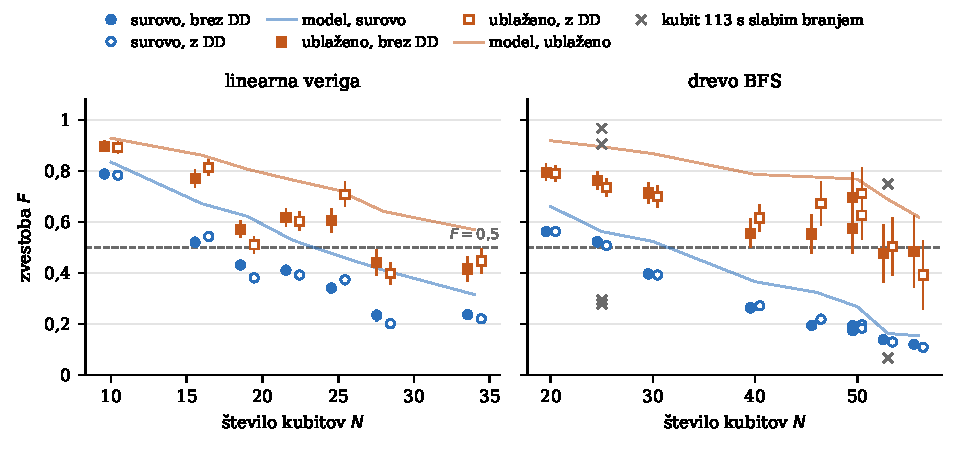
\includegraphics[width=0.98\textwidth]{ghz_fn}
\end{frame}

\begin{frame}{Meja $N_{\max}$}
\centering
\begin{tabular}{lrrr}
\toprule
konfiguracija & brez DD & z DD & model \\
\midrule
veriga, surovo & 10--16 & 16--19 & 26 \\
veriga, z ublažitvijo & 25--28 & 25--28 & 33 \\
drevo, surovo & 25--30 & 20--25 & 33 \\
drevo, z ublažitvijo & 50--53 & 50--53 & 70 \\
\bottomrule
\end{tabular}
\par\bigskip
\begin{itemize}
\item Brez ublažitve: veriga $N_{\max}\approx 16$, drevo $N_{\max}\approx 25$.
\item Z ublažitvijo se meja verige dvigne za približno 9, drevesa za približno 25 kubitov.
\item Največ prinese zasnova vezja skupaj z ublažitvijo; DD meje ne premakne.
\end{itemize}
\end{frame}

\begin{frame}{Nepričakovano: branje kubita 113 se je poslabšalo}
\begin{columns}[T]
\begin{column}{0.46\textwidth}
\centering
\begin{tabular}{lrr}
\toprule
posel ob & $e_0$ & $e_1$ \\
\midrule
14:26 & 0,065 & 0,076 \\
14:32 & 0,063 & 0,080 \\
14:42 & \textbf{0,462} & \textbf{0,215} \\
\bottomrule
\end{tabular}
\end{column}
\begin{column}{0.5\textwidth}
\begin{itemize}
\item Objavljena kalibracija tega ni pokazala.
\item Kalibracija v vsakem poslu je to razkrila.
\item Dodatni posel brez kubitov 113 in 131: surovi $F$ pri $N=25$ z 0,28 na 0,52.
\end{itemize}
\end{column}
\end{columns}
\end{frame}

\begin{frame}{Dinamično razklapljanje: dobitek in izguba se izničita}
\centering
Veriga, surovo\par\medskip
\begin{tabular}{rrrrr}
\toprule
$N$ & $P$ brez DD & $P$ z DD & $C$ brez DD & $C$ z DD \\
\midrule
25 & 0,498 & 0,441 & 0,182 & 0,305 \\
34 & 0,395 & 0,296 & 0,078 & 0,144 \\
\bottomrule
\end{tabular}
\par\bigskip
\begin{itemize}
\item Pri verigi DD zmanjša $P$ na vseh 7 točkah in poveča $C$ na 5 točkah.
\item Pri drevesu je vzorec šibkejši.
\item V $F$ je 18 primerjav navzgor in 18 navzdol, brez stalnega učinka.
\end{itemize}
\end{frame}

\begin{frame}{Primerjava z modelom in objavami}
\begin{itemize}
\item Model je na vseh točkah nad meritvijo: 0,02--0,24 surovo, 0,02--0,30 z ublažitvijo.
\item Vzroka razlike z ublažitvijo nismo ugotovili.
\end{itemize}
\bigskip
\centering
\begin{tabular}{lrrl}
\toprule
vir & kubiti & $F$ & opomba \\
\midrule
Wei idr.\ 2020 & 18 & 0,517 & \\
Mooney idr.\ 2021 & 27 & 0,546 & ublažitev branja \\
IBM 2025 & 120 & 0,56 & napredne tehnike \\
\midrule
naše drevo & 25 & 0,522 & surovo \\
naše drevo & 30 & 0,713 & ublažitev branja \\
\bottomrule
\end{tabular}
\end{frame}

\begin{frame}{Omejitve in kaj ni delovalo}
\textbf{Omejitve}
\begin{itemize}
\item Vsi glavni posli v 26 minutah enega dne; razpršenosti med dnevi ne poznamo.
\item Meja je odvisna od postavitve: $N=50$ da 0,70 ali 0,58 z ublažitvijo.
\item Pri $N\approx50$ ublažitev dvigne $F$ z 0,19 na 0,70: neposreden dokaz prepletenosti imamo le brez ublažitve, do $N\approx25$.
\end{itemize}
\medskip
\textbf{Kaj ni delovalo}
\begin{itemize}
\item Izbira kubitov iz objavljene kalibracije (kubit 113).
\item Točki $N=64, 76$ po napovedi modela: pilot ju je ovrgel.
\item Simulacija MPS z dvokubitnim kanalom Krausa je obtičala.
\end{itemize}
\end{frame}

\begin{frame}{Zaključek}
\begin{itemize}
\item S 113~s procesorskega časa: $N_{\max}\approx16$ za verigo in $\approx25$ za drevo brez ublažitve, 25--28 in 50--53 z ublažitvijo.
\item Največ prinese zasnova vezja skupaj z ublažitvijo branja, DD meje ne premakne.
\item Model iz objavljene kalibracije meje precenjuje, kalibracija lahko tudi zamuja.
\end{itemize}
\bigskip
\textbf{Nadaljnje delo}
\begin{itemize}
\item Kratko merjenje napak branja tik pred izbiro kubitov.
\item Dinamična vezja z meritvami sredi vezja: priprava v konstantni globini.
\end{itemize}
\end{frame}

\end{document}
